\documentclass[9pt,aspectratio=169]{beamer}
\usepackage{tikz}
\usetheme{Boadilla}
\setbeamertemplate{navigation symbols}{}
\title{Message passing: experiments and bounds}
\subtitle{Generated interaction study}
\author{Research group}
\date{}
\year=2026\month=11\day=5
\newcommand{\fuzzlayerA}[1]{\textit{#1}}
\newcommand{\fuzzterm}[1]{\fuzzlayerA{#1}}
\newcommand{\fuzzpair}[2]{\fuzzterm{#1}: #2}
\newcommand{\fuzzunit}{steps}
\let\fuzzoriginalunit\fuzzunit
\newcommand{\fuzzcoefficient}{2}
\newcommand{\fuzzscale}[2][\fuzzcoefficient]{#1\,#2}
\definecolor{fuzzpaint}{RGB}{255,0,255}
\definecolor{fuzzsecond}{RGB}{18,137,67}
\tikzset{fuzzvertex/.style={draw,rounded corners=1pt,fill=blue!10,inner sep=1pt,minimum width=.35cm,minimum height=.25cm}}
\begin{document}
\section{Message passing}
\begin{frame}[t,shrink=5]{Message passing}{Composed dependencies}
\fuzzpair{Experiment}{Timing: 12\fuzzunit; estimate $\fuzzscale{x}+\fuzzscale[2]{y}$.}\par
{\renewcommand{\fuzzunit}{samples}\let\fuzzterm\textrm\fuzzpair{LocalScope}{Timing: 7\fuzzunit.}\par}
\fuzzpair{RestoredScope}{Timing: 11\fuzzunit.}\par
\begin{exampleblock}{Incremental analysis}
\begin{columns}[onlytextwidth,c]
\begin{column}{0.54\textwidth}
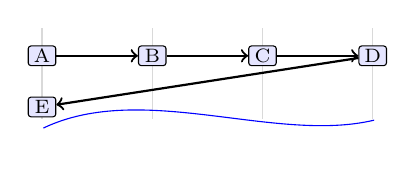
\begin{tikzpicture}[font=\scriptsize]
\begin{scope}[scale=1,rotate=0]

\foreach \x in {0,1,2,3} {\draw[gray!30] (\x*1.400,-.8)--(\x*1.400,.35);}
\node[fuzzvertex] (g3n0) at (0.000,0) {A};
\node[fuzzvertex] (g3n1) at (1.400,0) {B};
\node[fuzzvertex] (g3n2) at (2.800,0) {C};
\node[fuzzvertex] (g3n3) at (4.200,0) {D};
\node[fuzzvertex] (g3n4) at (0.000,-0.65) {E};
\begin{scope}[xshift=.5pt,yshift=-.5pt]
\draw<2->[->,thick] (g3n0) -- (g3n1);
\draw<2->[->,thick] (g3n1) -- (g3n2);
\draw<2->[->,thick] (g3n2) -- (g3n3);
\draw<2->[->,thick] (g3n3) -- (g3n4);
\draw[blue] (0,-.9) .. controls (1.260,-.3) and (2.940,-1.1) .. (4.200,-.8);
\end{scope}
\end{scope}
\end{tikzpicture}
\end{column}
\begin{column}{0.42\textwidth}
\begin{columns}[onlytextwidth,c]
\begin{column}{0.62\textwidth}
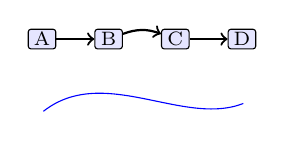
\begin{tikzpicture}[font=\scriptsize]
\begin{scope}[scale=1,rotate=0]


\node[fuzzvertex] (g5n0) at (0.000,0) {A};
\node[fuzzvertex] (g5n1) at (0.846,0) {B};
\node[fuzzvertex] (g5n2) at (1.693,0) {C};
\node[fuzzvertex] (g5n3) at (2.539,0) {D};
\begin{scope}[xshift=.5pt,yshift=-.5pt]
\draw<2->[->,thick] (g5n0) -- (g5n1);
\draw<2->[->,thick] (g5n1) to[bend left=20] (g5n2);
\draw<2->[->,thick] (g5n2) -- (g5n3);
\draw[blue] (0,-.9) .. controls (0.762,-.3) and (1.777,-1.1) .. (2.539,-.8);
\end{scope}
\end{scope}
\end{tikzpicture}
\end{column}
\begin{column}{0.34\textwidth}
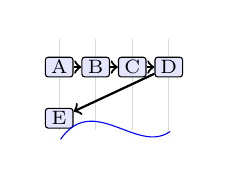
\begin{tikzpicture}[font=\scriptsize]
\begin{scope}[scale=1,rotate=0]
\clip (-.4,-1) rectangle (1.892,.5);
\foreach \x in {0,1,2,3} {\draw[gray!30] (\x*0.464,-.8)--(\x*0.464,.35);}
\node[fuzzvertex] (g6n0) at (0.000,0) {A};
\node[fuzzvertex] (g6n1) at (0.464,0) {B};
\node[fuzzvertex] (g6n2) at (0.928,0) {C};
\node[fuzzvertex] (g6n3) at (1.392,0) {D};
\node[fuzzvertex] (g6n4) at (0.000,-0.65) {E};
\begin{scope}[xshift=.5pt,yshift=-.5pt]
\draw<2->[->,thick] (g6n0) -- (g6n1);
\draw<2->[->,thick] (g6n1) -- (g6n2);
\draw<2->[->,thick] (g6n2) -- (g6n3);
\draw<2->[->,thick] (g6n3) -- (g6n4);
\draw[blue] (0,-.9) .. controls (0.418,-.3) and (0.975,-1.1) .. (1.392,-.8);
\end{scope}
\end{scope}
\end{tikzpicture}
\end{column}
\end{columns}
\end{column}
\end{columns}
\par
\begin{itemize}
\item<1-> 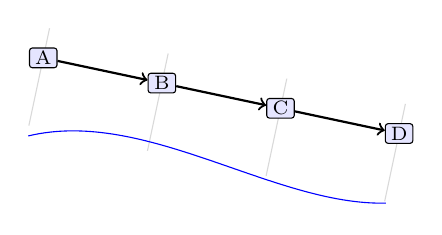
\begin{tikzpicture}[font=\scriptsize]
\begin{scope}[scale=1.1,rotate=-12]

\foreach \x in {0,1,2,3} {\draw[gray!30] (\x*1.400,-.8)--(\x*1.400,.35);}
\node[fuzzvertex] (g9n0) at (0.000,0) {A};
\node[fuzzvertex] (g9n1) at (1.400,0) {B};
\node[fuzzvertex] (g9n2) at (2.800,0) {C};
\node[fuzzvertex] (g9n3) at (4.200,0) {D};
\begin{scope}[xshift=.5pt,yshift=-.5pt]
\draw<2->[->,thick] (g9n0) -- (g9n1);
\draw<2->[->,thick] (g9n1) -- (g9n2);
\draw<2->[->,thick] (g9n2) -- (g9n3);
\draw[blue] (0,-.9) .. controls (1.260,-.3) and (2.940,-1.1) .. (4.200,-.8);
\end{scope}
\end{scope}
\end{tikzpicture}
\item<2-> \begin{tabular}{lrr}Method&Cost&Error\\\hline
Fresh0&6&0\\
Global1&6&17\\
Global2&9&16\\
Global3&1&6\\
\end{tabular}
\end{itemize}
\par
\[\begin{aligned}a+b&=c\\ d-e&=f\end{aligned}\]
\par
{\small\color{teal}\raggedleft
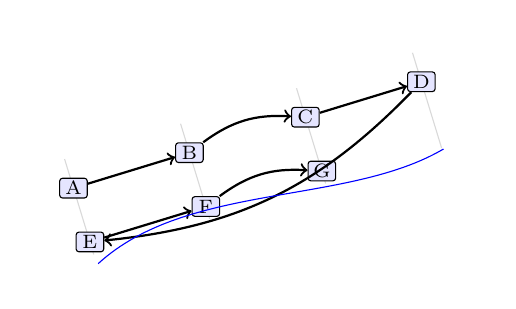
\begin{tikzpicture}[font=\scriptsize]
\begin{scope}[scale=1.1,rotate=17]
\clip (-.4,-1) rectangle (4.700,.5);
\foreach \x in {0,1,2,3} {\draw[gray!30] (\x*1.400,-.8)--(\x*1.400,.35);}
\node[fuzzvertex] (g13n0) at (0.000,0) {A};
\node[fuzzvertex] (g13n1) at (1.400,0) {B};
\node[fuzzvertex] (g13n2) at (2.800,0) {C};
\node[fuzzvertex] (g13n3) at (4.200,0) {D};
\node[fuzzvertex] (g13n4) at (0.000,-0.65) {E};
\node[fuzzvertex] (g13n5) at (1.400,-0.65) {F};
\node[fuzzvertex] (g13n6) at (2.800,-0.65) {G};
\begin{scope}[xshift=.5pt,yshift=-.5pt]
\draw<1->[->,thick] (g13n0) -- (g13n1);
\draw<1->[->,thick] (g13n1) to[bend left=20] (g13n2);
\draw<1->[->,thick] (g13n2) -- (g13n3);
\draw<1->[->,thick] (g13n3) to[bend left=20] (g13n4);
\draw<1->[->,thick] (g13n4) -- (g13n5);
\draw<1->[->,thick] (g13n5) to[bend left=20] (g13n6);
\draw[blue] (0,-.9) .. controls (1.260,-.3) and (2.940,-1.1) .. (4.200,-.8);
\end{scope}
\end{scope}
\end{tikzpicture}\par}
\par
\begin{columns}[onlytextwidth,t]
\begin{column}{0.54\textwidth}
\textrm{The next pass} must preserve the boundary conditions while revisiting dependent values.  The estimate is $\frac{a+b}{1+c}$.
\end{column}
\begin{column}{0.42\textwidth}
\textit{We compare the} proposed solution with a reference computed from the complete input.  The estimate is $x_i+x_{i+1}$.
\end{column}
\end{columns}
\end{exampleblock}
\par 
\begin{tikzpicture}[font=\scriptsize]
\fill<2-3>[fuzzpaint] (0,0) rectangle (.8,.3);
\fill<3->[fuzzsecond] (1,0) rectangle (1.8,.3);
\node[anchor=west] at (2,0.15) {Witness};
\end{tikzpicture}
\only<5>{}
\end{frame}
\renewcommand{\fuzzunit}{min}
\renewcommand{\fuzzcoefficient}{2}
\renewcommand{\fuzzterm}[1]{{\textrm{#1}}}
\section{Constraint propagation}
\begin{frame}[t]{Geometric uncertainty}
\fuzzpair{MacroStageB}{Timing: 12\fuzzunit, retained: 9\fuzzoriginalunit.}\par
{\renewcommand{\fuzzunit}{local}\fuzzpair{FrameLocal}{Timing: 5\fuzzunit.}\par}
\fuzzpair{FrameRestored}{Timing: 8\fuzzunit; estimate $\fuzzscale{x}$.}\par
\begin{columns}[T]\begin{column}{.46\textwidth}The final diagram records the order in which information crosses the partition.\end{column}\begin{column}{.46\textwidth}\begin{itemize}\item Input state\item Updated state\end{itemize}\end{column}\end{columns}
\end{frame}
\end{document}
